\documentclass{article}
\usepackage{geometry}                % See geometry.pdf to learn the layout options. There are lots.
\geometry{a4paper}                   % ... or a4paper or a5paper or ... 
%\geometry{landscape}                % Activate for for rotated page geometry
%\usepackage[parfill]{parskip}    % Activate to begin paragraphs with an empty line rather than an indent
\usepackage{graphicx}
\usepackage{amssymb}
\usepackage{amsthm}
\usepackage{amsmath}
\usepackage{mathrsfs}
\usepackage[french]{babel}
\usepackage{color}
\usepackage{listings}
\definecolor{javared}{rgb}{0.6,0,0} % for strings
\definecolor{javagreen}{rgb}{0.25,0.5,0.35} % comments
\definecolor{javapurple}{rgb}{0.5,0,0.35} % keywords
\definecolor{javadocblue}{rgb}{0.25,0.35,0.75} % javadoc

\lstset{language=Java,
basicstyle=\ttfamily,
keywordstyle=\color{javapurple}\bfseries,
stringstyle=\color{javared},
commentstyle=\color{javagreen},
morecomment=[s][\color{javadocblue}]{/**}{*/},
stepnumber=2,
numbersep=10pt,
tabsize=4,
showspaces=false,
showstringspaces=false}
\usepackage[utf8]{inputenc}
\newtheorem{theorem}{Théorème}
\newtheorem*{definition}{Définition}
\newtheorem*{exercice}{Exercice}
\hyphenpenalty=10000

\title{Secure Airport Tower\\Development Journal}
\author{frederic.jacobs@epfl.ch\\ hantao.zhao@epfl.ch}
\begin{document}
\maketitle 
This journal is a week-by-week development journal. We'll highlight our progress and the reason why we chose to do it this way.

\section{Week One}
This week we were given the topic of the ITP and we mostly documented ourselves about how it should work. 
Here are the main areas of focus of our research and coding : 
\begin{enumerate}
\item \emph{Versioning} : We started by setting up a versioning system for easier collaboration. Instead of sticking to SVN we decided use GIT hosted on GitHub.There are many reasons to explain this decision but we'll highlight here only a few. We really fancy the social features of GitHub for collaboration. GitHub Issues makes it easier to report bugs and to fix them. Git is also way simpler to set up than SVN. The branching of Git makes it way easier to work on different branches and then merge them with the master at a further stage. We set it up as a private repository according to the requirements of this course.
\item \emph{Unit Testing} : We added the \verb JUnit  framework to our new Eclipse project for Unit Testing and ran a few tests to get used to the framework and assertions. 
\item \emph{Encryption}: We were given a lecture by Prof. Telatar about RSA encryption. We coded two custom RSA classes (KeyPair and KeyGenerator). We couldn't manage to find time to code these classes during the project time because some method names in the test weren't straightforward. 
\end{enumerate}
Fortunately we ended up doing this before starting the next weeks ITP. We also found some time to comment the classes according to the JavaDoc. 

\section{Week Two}
Week Two was all about defining the messages. We first defined all the \verb Messages  subclasses in the same file which ended up being a bad idea for OOP encapsulation. We wrote a \verb .java  file for each of the messages and bundled them in a \verb messaging  package. 
So we ended up rewriting all these messages later that week which allowed us also to adapt our constructors according to the ones in the Unit test. We also implemented a \verb PriorityQueue  which we got to work very easily but optimized it when we had the network support. What the messages were doing was crystal clear in our heads but how the \verb Tour.java  was going to handle is with the priorityQueue remained a big mystery that we only understood later. \newline 

In ITP-02, we were asked two questions. 
\begin{enumerate}
\item Is it a good idea to use a superclass to define Messages ?
\item Why is it an abstract class ?
\end{enumerate}
In a object-oriented universe like Java, we like to model things hierarchically. We want all possible types of messages to have a behavior or to have some instance variables therefore defining a super-class Messages makes a lot of sense. We were asked to have these instance variables in each Message Type so we implemented these in our super-class.

\begin{lstlisting}
byte[] planeID;  //The unique identifier of the plane
int length; //Length of the message
int priority; //Priority in PriorityQueue
int posx; //Positioning data 
int posy;
MessageType type; //Type of Message
\end{lstlisting}

The reason why we want this to be an abstract class is really straightforward. We defined a Message super-class because we expect messages to behave a given way but we also want these messages to have a type. All messages will inherit these attributes from the super-class but the super-class won't be instantiable to assure we call the right constructor when creating a message with a certain type. The keyword \emph{abstract} does exactly this. 


\section{Week Three}
During this third week, we came back to the \emph{encryption} and we made two new classes. \verb RSAInputStream   (inheriting \verb InputStream  ) and \verb RSAOutputStream  (inheriting \verb OutputStream  )  to support inputs and outputs of encrypted data and messages. These classes were built pretty quickly and we focused more on the \verb DataFile  class which was way more difficult to code. To start with, we choose to use a \verb HashMap  for rebuilding files. Splitting files was easy but rebuilding them once splited took some extra time. We adapted the Unit Test to work correctly but we definitely need to come back to this file to improve it.

\section{Week Four}
This week we were given a two weeks assignment. We started in the morning refactoring our project with more consistent naming of the packages. We also worked on fixing the \verb DataFile  class that needed improvements. Then we started working on a new networking package defining the Sockets needed for messaging. It took us some time to realize we actually needed one socket per plane from a Tower's perspective. We started coding this but forgot multi-threading which made the whole program very unresponsive. That week has been very busy for us ("Voyage d'études") and other assignments. So we left it like until the next Tuesday.

\section{Week Five}
We made some great progress. The networking part finally got cleaner and we are now trying to put everything together. In the meanwhile we used a external library to make an OAuth on Twitter. We made a static class that can send tweets. Hence, the keys are set in a configuration file and can't be set differently at the time. Over the weekend we made some great progress. The networking discovery now works and the handshake is correctly done. Our class \verb DataFile  now works with the given tests. We still want it to become more robust and we'll  be looking into implementing a better hash verification implementation because it is very tricky on how it behaves.

\section{Week Six}

The midterm return is coming up, so we need to try our best to combine our packages and build a reliable connection not only just between the tower and the plane, but also between our packages and classes. We can already hear and talk to any given airplane by using our RSA encryption streams.  This weekend we worked on adapting the encrypted communication to the given test plane. We decided to finish the \verb DataFile  during the vacation. 
On the other hand, we are done with Twitter Integration. Sending a Tweet is easy and can be done in a single line of code. We finalized the JournalGUI but definitely needs some improvements. 

\section{Midterm Conclusion}
When starting new ITPs we did really misunderstand the expected way of coding and wasted lots of time coding it the wrong way or fixing little mistakes. The biggest difficulty we faced so far was putting all the separate pieces together. Making the packages work together was tricky. An example of this is the \verb DataFile  . It works quite well when we run it with our own tests but it doesn’t work for the demo planes. The good news is that basic functions are working and according to the assistant the main architecture is satisfactory. Meanwhile we would love having some suggestions about architecture so we can make it more robust after the midterm. 

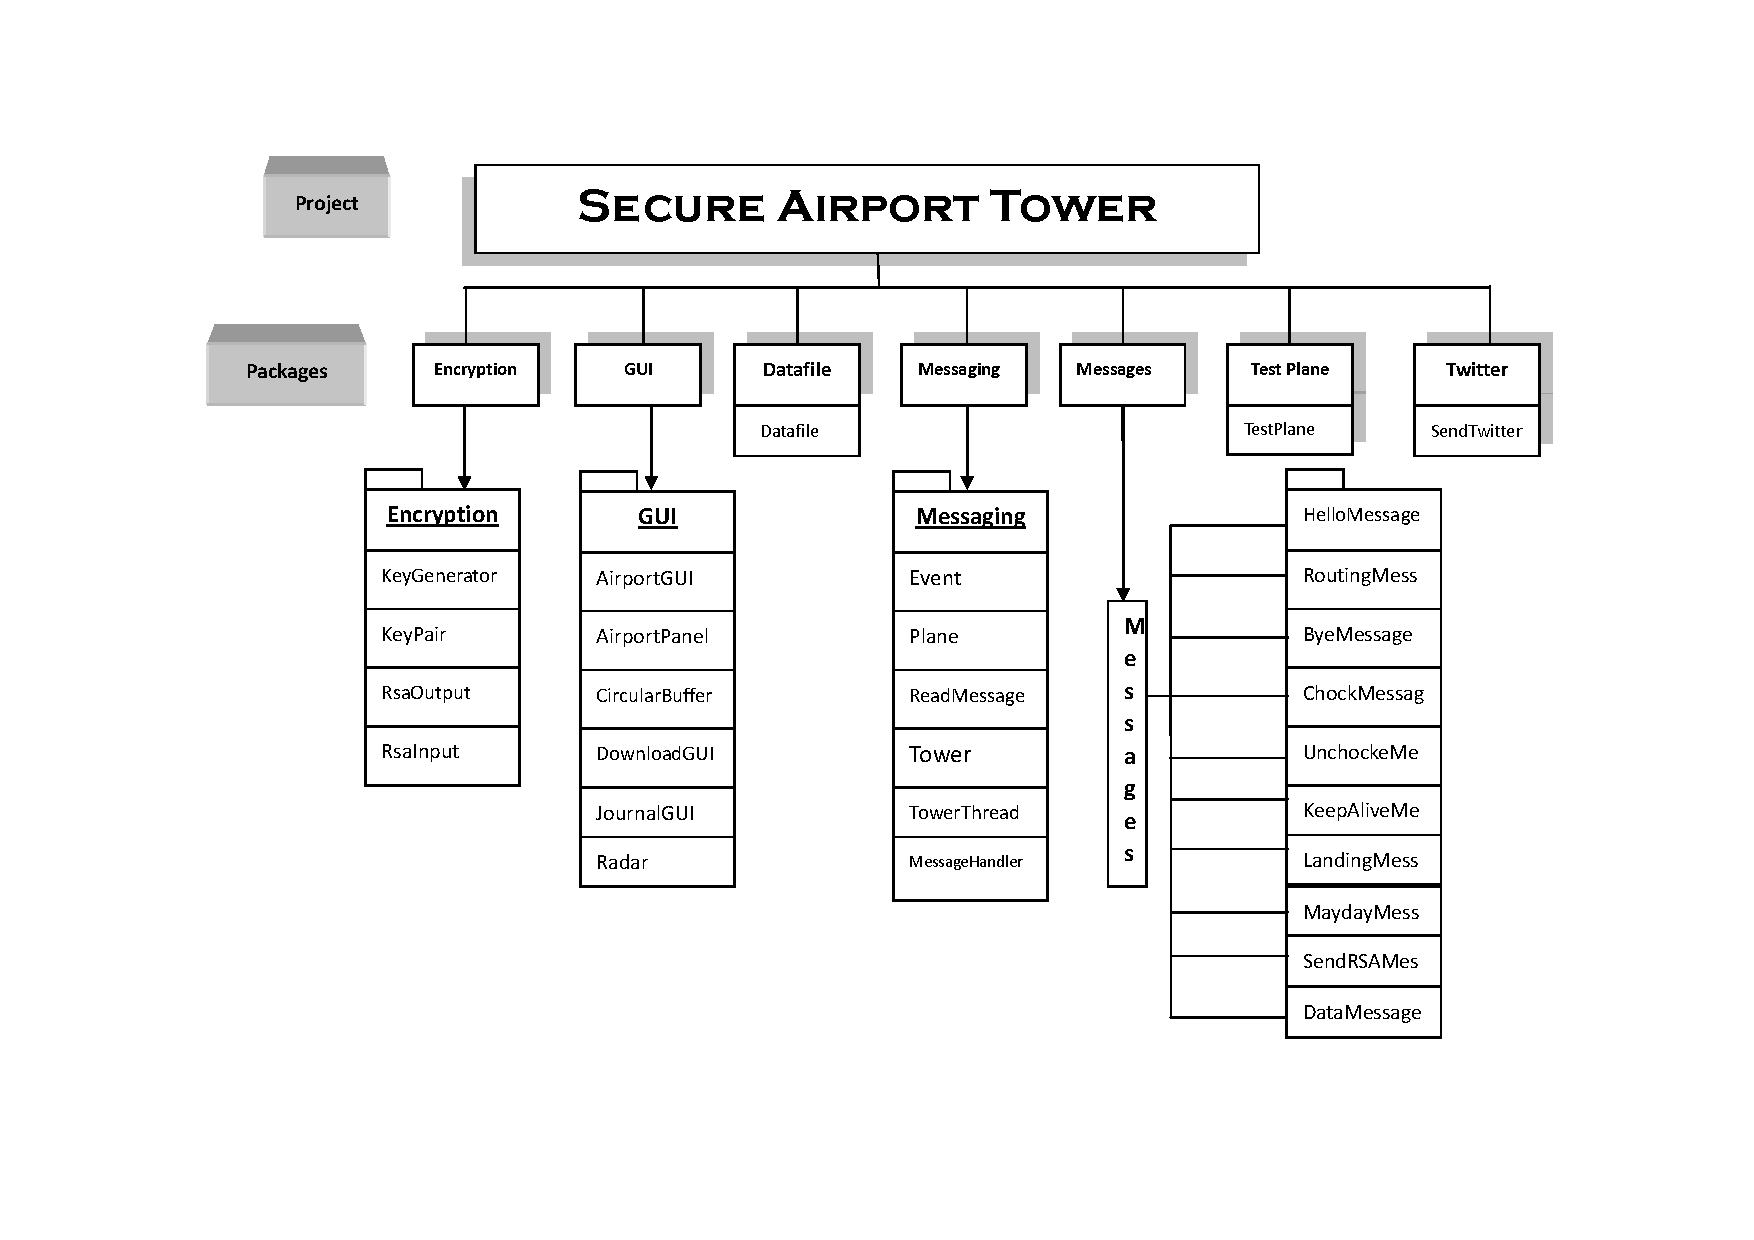
\includegraphics[scale=0.45]{UML.pdf}
\newpage

\section{Week Seven}
During this week we didn't make much progress. It was a very busy week for the both of us. We did however did some refactoring including the way we are handling the journal and logs. We did create an event class that is just a container for a single event and that allows us to log each message easier. Over the weekend we did make some progress on programming the planes and finalizing the the logging events.
\section{Week Eight}
We started working on the things that were still missing (Airport GUI and Routing Messages) to catch up with the ITP-06 and will be starting with ITP-07 as soon as possible. We are not up-to-date but we are not left behind either. We'll try to catch up over the weekend since this week is less busy than the preceding one.

\section{Week Eight}
During this week we've been focusing on the GUI improvements and fixing of bugs in the DataFile that caused files never to be transfered correctly or not in an optimized way. We also added the Choke/Unchoke function in the GUI that was missing. Some progress has been made on routing and the coding of the planes but both things still require some additionnal improvements.

\section{Week Nine}

We added the types of plane to our customized plane to have advanced compatibility with the given planes and programming guidelines. Routing has been partially implemented but remains tricky and there is progress to made. We also got our innovation approved. We'll be working on a JSON API to get data from the Airplane tower over HTTP. The following weeks will be very busy. We still have some features to implement (ITP-7) and we have a lot of work to do on our innovation. We'll try our best to get as much as possible working in a clean and clever way.

\end{document}


